\documentclass[11pt,journal]{IEEEtran}
%\usepackage{hyperref}
%\usepackage[breaklinks]{hyperref}
\usepackage{breakurl}
\usepackage{url}
\usepackage{listings}
\usepackage{courier}
\usepackage{graphicx}
\ifCLASSOPTIONcompsoc
% IEEE Computer Society needs nocompress option
% requires cite.sty v4.0 or later (November 2003)
\usepackage[nocompress]{cite}

\else
% normal IEEE
\usepackage{cite}
\fi

\hyphenation{op-tical net-works semi-conduc-tor}


\begin{document}
	\title{Expanding the proof rule base and tactics of AtelierB automated prover - Research Proposal}
	
	\author{Agata~Borkowska,~UID: 1690550,~\IEEEmembership{MSc in Computer Science,~University of Warwick}% <-this % stops a space
		\protect\\
		\thanks{}}
	
	% The paper headers
	
	\markboth{}%
	{ \MakeLowercase{\textit{}}: }
	
	\IEEEcompsoctitleabstractindextext{%
		\begin{abstract}
			%\boldmath
			AtelierB is a tool for formal software development through refinement, using the B-method. It incorporates an automated prover, which has been recognized as the most thorough prover for B set theory, and has been used as a basis for many others. Nevertheless it has multiple shortcomings. Various approaches have been suggested and taken to improve its performance, including extensions to the proof rule base, created by the users. In this work we aim to create such an extension, ensuring that all added rules are sound and well-reasoned. We also aim to identify any limitations of this approach. The secondary goal is to improve the robustness of the software without straying from pure B method, and taking into account the ease of use. As a metric of our success, we use the benchmarks proposed by Conchon and Iguernala\cite{survey}.
	\end{abstract}
	\begin{IEEEkeywords}
		B method, formal verification
	\end{IEEEkeywords}}
	% IEEEtran.cls defaults to using nonbold math in the Abstract.
	% This preserves the distinction between vectors and scalars. However,
	% if the journal you are submitting to favors bold math in the abstract,
	% then you can use LaTeX's standard command \boldmath at the very start
	% of the abstract to achieve this. Many IEEE journals frown on math
	% in the abstract anyway. In particular, the Computer Society does
	% not want either math or citations to appear in the abstract.
	
	% Note that keywords are not normally used for peerreview papers.
	
	% make the title area
	\maketitle
	
	
	% To allow for easy dual compilation without having to reenter the
	% abstract/keywords data, the \IEEEcompsoctitleabstractindextext text will
	% not be used in maketitle, but will appear (i.e., to be "transported")
	% here as \IEEEdisplaynotcompsoctitleabstractindextext when compsoc mode
	% is not selected <OR> if conference mode is selected - because compsoc
	% conference papers position the abstract like regular (non-compsoc)
	% papers do!
	\IEEEdisplaynotcompsoctitleabstractindextext
	% \IEEEdisplaynotcompsoctitleabstractindextext has no effect when using
	% compsoc under a non-conference mode.
	
	
	% For peer review papers, you can put extra information on the cover
	% page as needed:
	% \ifCLASSOPTIONpeerreview
	% \begin{center} \bfseries EDICS Category: 3-BBND \end{center}
	% \fi
	%
	% For peerreview papers, this IEEEtran command inserts a page break and
	% creates the second title. It will be ignored for other modes.
	\IEEEpeerreviewmaketitle
	
	
	
	\section{Introduction}
	\IEEEPARstart{T}{he} aim of formal specification and verification is to ensure the correctness of software. While overall less popular than quality assurance through testing, it is most commonly used in safety-critical areas, such as air traffic control, railway routing, or medical cyber-physical systems, or where testing is too costly or puts the users at risk. It allows for certifying that a given piece of software works as intended, and is error-free.
	
	In some industries, such as railway, it is demanded by the regulations to provide a certificate of correctness for any piece of software. While not required, it is strongly suggested to use formal verification methods, such as B or Z, and indeed they make satisfying the regulations easier.\cite{railway standard}
	
	\subsection{The B-method}
	Various methods and approaches have been developed. In this project, we shall focus on the classical B-method, allowing for formal specification through refinement of abstract machines. In the earliest stages of the development process, an abstract machine is created, that satisfies the requirements. It is a construct based on 1\textsuperscript{st} order logic and set theory. At this point, there is no reasoning about the order of operations and timeline - no loops, no sequential actions. Additionally the machine may, and often will have some nondeterministic elements. 
	
	The abstract machine is then refined step by step, until the nondeterminism is eliminated. The final stage of the refinement process is the implementation, which is a much more concrete description of the system, ready to be translated into code. Thus it has to be entirely deterministic, and use simple data types, such as numerical values or arrays, but not sets. While limiting, it brings us very close to the actual coding, and in fact some tools are capable of code generation from the implementation machine.
	
	The B-method allows us to do much more than turning an initial specification into an auto-generated (and because of that often low quality) code. It gives us means of documenting the whole software development process, and certifying that the final product indeed meets the requirements.
	
	\subsection{AtelierB tool}
	The tool to support all stages of software development with B-method is AtelierB, created by ClearSy. In particular it includes a powerful automated prover. We will inspect it and the proof process very closely, as the work in this project is expected to rely on it entirely.
	
	After creating the specification, we can generate proof obligations (POs). They are statements about the consistency of the types of variables, well-defineness and other things that are implied by our definitions or methods. In a correct piece of software, all of the POs should be demonstrated to hold. If there is a PO that cannot be proved to hold by any means, it indicates that there exists an error in the specification.
	
	An easy example to demonstrate it is a bag, from which we pick an item one by one. The operation to pick an item guarantees some return value, so a proof obligation generated by the tool may require us to check that the bag is never empty when this operation is called.
	
	It is expected that about 75\% of the POs will be demonstrated automatically, and only 5\% of them will require more than 10 s (i.e. proof force 1 or higher)\cite{Prover guide}. The remaining POs will need user input to be discharged. This is done through the automated prover, with the user chosing which rule or tactic to apply, simplifying the hypothesis and in general nudging the prover and pointing it in the right direction.
	
	
	\subsection{Limitations of the prover}
	It is important to understand that the prover can only generate proof obligations and demonstrate that they are satisfied, but is incapable of proving that they are not - this problem is undecidable. In other words, each proof obligation can only be proved or unproved, and the latter can happen for one of two reasons. It is quite likely that a PO is true, but the program cannot prove it automatically because of its complexity. However, the unproved obligations also include the ones that are false and point to errors in the specification. 
	
	Finally, it has to be stressed that adding user-created rules is not advised, and should be avoided, however that may not always be possible. The tools available are not perfect and additionally may not be tailored to the particular scenario. All added rules must be proven to be correct, before one can rely on them. Although the prover has some capability for demonstrating a rule by reducing and rewriting it into a simpler form, new rules often have to be validated by hand. There is nothing stopping users from adding incorrect rules, and especially ones that do not deal with all possible test cases are often not shown to be false easily.
	
	\section{Related Works}
	
	\subsection{Applications of B-method}
	Although it may seem purely theoretical at first, the B-method has industrial applications, especially in safety-critical areas. It is3 commonly used in European Railway industry, from traffic management systems to developing platform door controllers\cite{Door controller}.
	
	An example of using classical B-method in a large scale industrial project is given by F.~Badeau and A. Amelot\cite{airport shuttle}. They have aided Siemens Transportation Systems to develop an shuttle rail service at Paris-Charles de Gaulle Airport. The fully automatic metro line began its operation in April 2007, and has been functioning since then, with one more metro line added in June 2007.
	
	This example is the most illustrative one, as the authors provide a clear breakdown of what work went into proving both the abstract and the concrete models. They have generated over 43 thousand proof obligations, 97\% of which were proven automatically. While it is a quite good result, at this scale it leaves over 700 POs to be proven by hand, and according to the authors, their average rate was proving manually around 15 obligations per day. It demonstrates just how time consuming it is to work with a tool that is not as automatic as one claims to be.
	
	More importantly, the authors had the need for 290 new proof rules. They have discovered that the Predicate Prover in AtelierB was very useful in validating them. 84\% have been done by the tool, however the remaining ones have consumed many man-hours to validate. It is a pity that more details on this are not provided.
	
	In the formal model of railway stations proposed by K.~Reichl \emph{et al.}\cite{Railway routing}, an evolution of B-method called Event-B is used, as it allows for modelling systems as a whole, including hardware. Nevertheless the underpinning theory and relying on first order logic and set theory is common to both B and Event-B. Event-B also requires Rodin tool, rather than AtelierB, however in their work, the authors have used AtelierB prover in addition to Rodin's one.
	
	K. Reichl \emph{et al.} have achieved a similar proportion of proved POs to Badeau and Amelot - 97.6\% of their POs were discharged  by the prover. This number seems to be quite consistent. E. Bernard \emph{et al.} in their B model of GSM 11-11 smart cards had 377 proof obligations generated, and all but one of them were discharged automatically (the last one requiring the interactive prover)\cite{GSM}. D. Mentr\'{e} \emph{et al.} also got over 90\% of POs discharged by the prover in their use of pure Atelier B for benchmarking.\cite{discharging}
	
	Unfortunately, in neither of this paper it is stated if any measures were taken during the writing of the specification, to make the proof process easier. For example, it is possible that certain constructs were avoided, or logical statements were simplified from the start. Also, it is possible that the majority of the POs generated are very similar and simple, such as type checking for each variable, and once one of them is discharged, the rest will follow in a similar fashion.
	
	
	\subsection{Methods for verifying provers}
	
	As mentioned earlier, adding proof rules requires a thorough verification of them by the user, and is generally discouraged. However it may be unavoidable, and event more importantly one might ask why we trust the rules provided by Atelier B. 
	
	There are multiple automated theorem provers and proof assistants, not made specifically for the B-method. One of the more common ones is Coq. It has been developed over 20 years ago, and have been used to formalize B semantics since then.\cite{Coq and PVS}.
	
	There was also an attempt by P. Chartier to formally validate B using Isabelle/HOL\cite{Isabelle}. The aim of this work was to verify methods of automatically generated proof obligations and check their consistency.
		
	Both Coq and Isabelle/HOL use embedding to reason about B. In the case of Coq, the method lies between deep and shallow embedding, where B is translated into objects that are semantically equivalent, however not all of the properties of B can be stated in the target langauge\cite{Coq and PVS}. In the case of Isabelle/HOL, only semantic embedding of the core elements of B is described.
	
	Zenon theorem prover has been developed more recently with first order logic in mind.\cite{Zenon} It uses truth trees, which make it much easier to add rules outside the core collection, such as is often required in B, and to check that the proof is correct. It generates proofs that can be then analysed by Coq.
	
	M. Jacquel \emph{et al.} have formally developed a framework based on Zenon, for verifying proof rules that are beyond the capabilities of the Atelier B's prover.\cite{embedding and theorem proving}. On top of that they very clearly describe the step-by-step process they have used in developing B proof rules, and present the benchmarks used. Both of these aspects of their work can become very helpful as we work on this project.
	
	Another part of verification using B is demonstrating the generated proof obligations. Ideally we want to prove all of them to hold, however this problem is undecidable.
	
	The currently predominant approach to improving the power of the interactive prover in Atelier B is using SMT solvers. Satisfiability Modulo Theories are a generalised form of SAT, taking into account some underpinning theory for the formulae. This results to generally undecidable problems being much simpler in a particular scenario.\cite{SMT handbook}
	
	D\'{e}harbe explains in detail how to use SMT to discharge proof obligations for B and Event-B, including those that are not limited to simple types and logic constructs. While his work focuses primarily on Event-B and Rodin, he speculates that it should be possible to apply his work to classical B and Atelier B in a very similar way.\cite{SMT} This is an avenue we would definitely want to explore in our project.
	
	Multiple SMT solvers exist, the most popular one being Why3. D. Mentr\'{e} \emph{et al.} have developed a method to use them to discharge proof obligations that Atelier B cannot cope with. More specifically, they rigorously translate B proof obligations into Why3. It required modelling the B set theory in Why language. Unfortunately, their work is incomplete, and their are some questions about confidence in their embedding of B into Why3.
	
	Alt-Ergo is another solver, which has been used to discharge Atelier B's POs.\cite{Alt-Ergo} Alt-Ergo is an open source project by Conchon and Igernelala. The focus of their work is efficiency and improvement of heuristics. Interestingly, they have discovered that an SMT solver on its own will not do better than the Atelier B's interactive prover. It required some tuning specifically for B method, after which there was a noticable improvement in performance.
	
	It should also be pointed out that the Atelier B Maintenance edition includes a tool for validating mathematical rules. Unfortunately we are unable to gain access to it. It is not a great loss however, as in this project we will focus on other aspects of the tool as well as the proof rule base, and additionally there are almost no references to the tool that assess its usefulness.
	
	\subsection{Plugins, extensions and other software}
	
	A very common approach to improving the provers, be it for the classical B-method or Event-B, is to create a plugin or an extension to AtelierB and Rodin respectively. While this is not the aim of the project, and we make an attempt to improve the tool by means available through them, some of the methods are portable and give us an idea of how to approach certain problems. Additionally we look at the problems the creators of the extensions came across, as a warning and inspiration.
	
	A reason for creating extensions and modificatons to the software was discussed by M. Leuschel \emph{et al.} in their paper on case studies of large scale models of metro lines in various cities\cite{San Juan metro}. They found that AtelierB was not optimised very well and tended to run out of memory, when working on real-life models.
	
	Other reasons include lack of functions that cover testing and animating the models in Atelier B and perhaps most importantly Atelier B's prover not changing much over the last two decades, despite advances in the methods for automated theorem proving.
	
	The most popular program to aid with development using Atelier B, is the ProB tool, which animates the models and tests them on the case by case basis.\cite{ProB} It has also been used in industry alongside Atelier B \cite{San Juan metro}. It is often called a 'disprover' for Atelier B's prover. The name is perhaps misleading; while we cannot prove that a statement is false in the same way we prove it to hold, we can disprove it by counterexamples, and this is exactly what ProB does.
	
	ProB allows for enumerating the states of the machine, and simulating the operations. It is also quick to detect when the rules are violated, thus saving time that otherwise would be wasted on futile attempts to demonstrate the false PO with the interactive prover of Atelier B.\cite{Prob intro} However, as a result of the enumeration, it will not provide counterexamples in the cases when the cardinality of a set is not fixed, which is the case with deferred sets, or when a PO contains an integer which has a value independent of the rest of the statement. Therefore ProB cannot be used as a prover, but only as a tool to find counterexamples\cite{ProB for eventb}.
	
	Medeiros and D\'{e}harbe\cite{BEval} have made an attempt to create a plug-in for Atelier B to combine it with ProB. It allows for communication between the two tools, such as picking expressions from Atelier B and passing them to ProB, then generating further (and hopefully simpler) statements in B notation, which may be discharged by the interactive prover. It is even intended to generate proof rules that can be automatically used by either prover. The latter is useful especially for well-definedness POs, which Atelier B's interactive prover does not discharge for unclear reasons.
	
	The BEval plugin is available online and is completely open source, and it would be interesting to experiment with it, especially that the authors say very little about the limitation of their work. They only mention expected problems caused by the dissimilarities between the Atelier B and ProB syntax.
	
	Another project worth noting is called BWare, created by D. Delahaye \emph{et al.}.\cite{BWare} As it is very recent, the presented results are preliminary. They have opted to use multiple tools to achieve their end goal of discharging more POs than the interactive prover of Atelier B is capable of. The foundation of their project is the Why3 platform, and used Alt-Ergo SMT solver, having also considered Zenon.

	While in this project we want to avoid creating or using extension, inspecting the existing ones more closely will definitely be helpful. They can serve as an inspiration or help with testing and benchmarking.
	
	\subsection{Shortcomings of Atelier B}
	
	As mentioned before, M. Leuschel \emph{et al.} were very critical about Atelier B, and it is worth looking closely at the issues they have raised. Their main problem with the tool and the focus of their paper was lack of optimisation, however they listed others as well. They noted that in the case of undischarged POs, it was "difficult to find out why the proof has failed".
	
	An important warning to be taken out of their paper is concerned with the \textsc{Definitions} section of an abstract machine. Their behaviour is almost identical to that of macros, and may be prone to errors if not inspected properly. The example given in the aforementioned paper is a definition \texttt{sum(x,y) == x+y} which AtelierB will use as is. Thus an expression \texttt{sum(1,1)*2} will result in \texttt{1+1*2}, which is clearly not the intended outcome. [NOTE: WILL TRY TO REPLICATE ON LAB MACHINES. NEED PROB]
	
	The issues mentioned above are quite general and in line with our own experience. We will not go into the details of bugs raised in the paper, as the authors have been using Atelier B version 3.6.2, while the one we use 4.2.1, released in December 2014. According to the release notes, more than 150 bugs have been fixed since the previous version. However, no list of known bugs and issues has been found for the newest version.\cite{release notes}
	
	Another issue is mentioned by Medeiros and D\'{e}harbe\cite{BEval}. They point out that Atelier B is falling behind the developments made by researchers in the area of automated theorem proving. It is unsurprising, as the tool's development process is slow due to the need for certification of every update, without which it could not be used in an industrial setting.
	
	While we will not aim to fix these issues, it is necessary for us to be aware of them. It should also be pointed out that despite all its shortcomings, Atelier B is the most popular and the best developed tool. It has been around for over 20 years, and has the largest user base out of all software for development in B. The plugins and software listed in the previous sections, although may have better design and functionality, are not yet up to industry standards, while Atelier B has been certified to be up to it.
	
	On top of that all of them rely on on Atelier B. All of the papers discussed in this section mention using Atelier B for the first pass of type checking and discharging proof obligations. It is at the core of the formal specification of many industrial projects. Therefore we will focus on this tool only, and avoid introducing changes that would result in the same problem as the custom extensions - lack of resources for development leading to inferior quality.
	
	
	
	\section{Project Aims}
	In this project we shall focus on the AtelierB automated prover. The key aim of the project is to push it to its limits, without creating ay plugins or extensions. We are interested to see how much can be achieved with the prover on its own.
	
	We shall also look at different ways of writing and phrasing the specification to make it more prover-friendly. Some of the questions we would like to answer are: are there any ways of expressing commonly found points that will make them faster to prove automatically? How much impact does the complexity of expressions have on the prover's ability to discharge POs? If any of the items found above are non-intuitive, can we create tactics that will bridge the gap between the prover's ability and the user's way of thinking?
	
	A secondary aim of the project is to analyse the user-friendly aspects of the AtelierB tool or lack thereof. The difficulty to understand why a proof has failed was brought up by M. Leuschel \emph{et al.} in their broad case study\cite{San Juan metro}, among others. 
	
	It is expected that over the course of this project, new questions and ideas will arise. Some, but not all may be pursued, while others will be identified as areas for further research.
	
	\subsection{Choice of Scenarios}
	To recognize the most commonly problematic proof obligations, we will collect a few scenarios created by various research groups or companies. This will ensure that the issues with the prover will not be user-specific. 
	
	The most important criteria in choosing third party models will be created using only B-method (and not extensions to it, such as Event-B), and that they will be well-documented, especially in terms of tools used for verification.
	
	As it has been identified in the literature review, the industry that most commonly uses the B-method in practice is Railway, and there are models available online [cite]. However, it is well within the scope of this project to assess if there are problems common to different scenarios.
	
	Thus, the railway industry will be the primary focus, however we will compare the improvements made across a range of scenarios, not limited to this area.
	
	\subsection{Expected learning outcomes}
	The key outcome is a deeper understanding of methods and tactics for formal verification and validation through refinement, the underlying theories and the reasonings. 
	
	Additionally, we hope to become very familiar with writing formal specification in B, knowing the pitfalls and gaining practice and experience.	
	
	We hope that the outcome of this project will help future students and other people hoping to understand the workings of Atelier B's automated prover.
		
	\subsection{Methodology}

	Given that the aims of the projects can be summarised as "explorations and discovery", the overall approach to the project will be agile. 
	
	To ensure that the methods chosen are not misleading or very suboptimal, we will cross-reference them with existing works, which will serve as inspiration. However, rather than repeating what other people have done, we will focus on synthesizing their methods and experimenting with various combinations thereof. 
	
	We will also use a range of scenarios, from some 
	
	\section{Project Management}

	
	\subsection{Timeline}
	Key dates, as listed by the CS907 Dissertation Project website, are:

	\begin{figure*}[]
		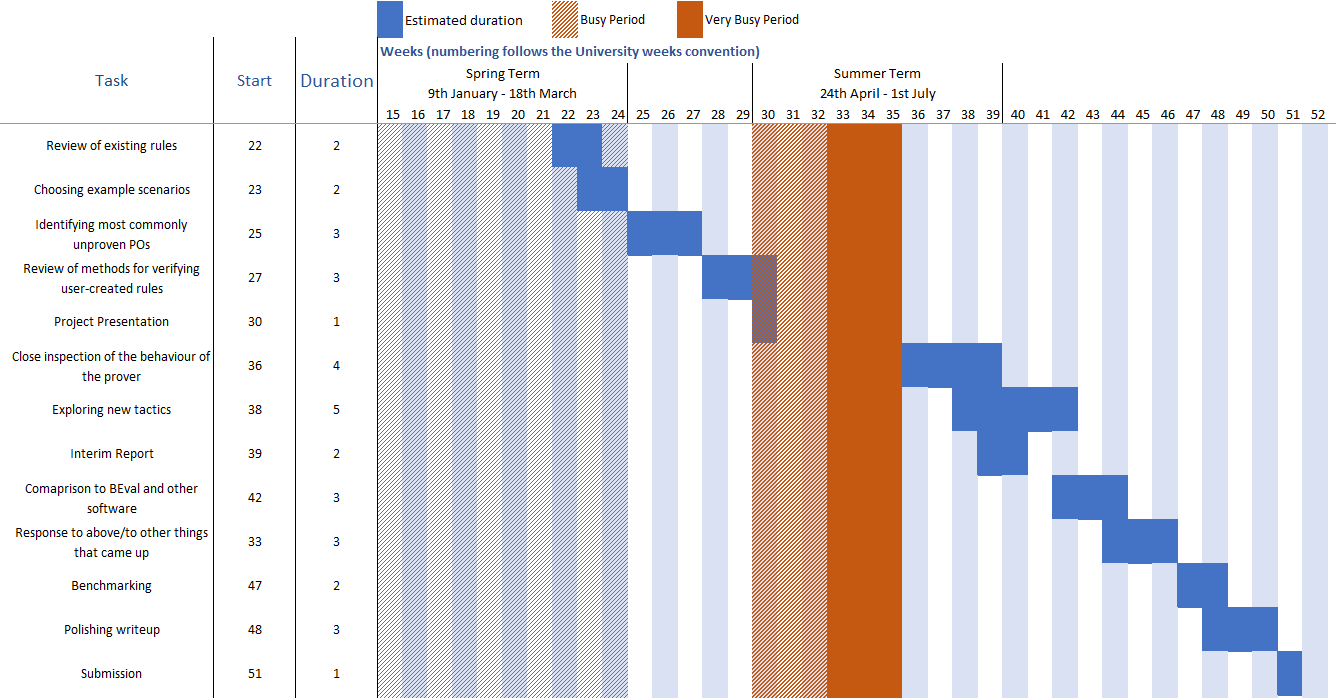
\includegraphics[width=\textwidth]{gantt_chart.png}
		\caption{Gantt chart with the rough timeline of the project}
	\end{figure*}
	\begin{itemize}
		\item \textbf{19\textsuperscript{th} January:} Registration of dissertation topics
		\item \textbf{16\textsuperscript{th} February:} Submission of project proposals
		\item \textbf{24-28\textsuperscript{th} April:} Project presentations
		\item \textbf{6\textsuperscript{th} July:} Submission of interim reports
		\item \textbf{14\textsuperscript{th} September:} Submission of dissertation
	\end{itemize}
	

	It is also important to take into account dates of terms, which are 9\textsuperscript{th} January to 18\textsuperscript{th}March for the Spring Term, and 24\textsuperscript{th} April to 1\textsuperscript{st} July for the Summer term, with the university examinations commencing on or after the 15\textsuperscript{th} May, and being spread over a period of about two weeks. Therefore, it is to be expected that little progress will be made during Spring Term and especially in May, with the bulk of the work being done over holiday and after the examination period.
	
	The Gantt chart in Fig. 1 shows an estimate of the project's timeline. 	


		
	\subsection{Progress}
	To make sure that a sufficient progress will be made, some of the actions listed above will be identified as milestones. 
	
	Additionally, regular meetings with the Supervisor have been scheduled to monitor progress.  
	
	\subsection{Constraints and Risks}
	\subsubsection{Copyrights for AtelierB software}
	Atelier B is a closed source project, however it is distributed free of charge, for any purpose including teaching and research. ClearSy does not forbid users from making modifications to their software, however any modified software will be excluded from their maintenance service policy.
	
	The maintenance edition of the software includes a tool for proving mathematical rules. It could potentially be helpful to have access to it in the project, however as of now we do not have the means to gain access to it.
	
	\subsubsection{Bugs in AtelierB and lack of responses from ClearSy}
	It should be highlighted that we have not found a list of bugs and known issues with any version of Atelier B. The company blog includes a page on it, however it has not been updated since August 2012, and the content (which could be of some use, even if it were outdated) does not load.\footnote{\url{http://tools.clearsy.com/tools/bug-status/} Note the first comment about the size of the table.} ClearSy has been contacted for us to gain access to the updated information.
	
	Thus our main source of informations about issues with the software is academic publications and unfortunately word of mouth. This is not reliable at all. It is also worth pointing out, that despite multiple attempts to contact ClearSy about bugs and other problems found in Atelier B since October last year, we had no response so far.
	
	If any bugs are encountered during the work on this project, they will be reported to ClearSy as well as highlighted in the project. 
	
	\subsubsection{Requirement for knowledge outside the subject area}
	The B-method relies heavily on first order logic and Zermelo-Fraenkel set theory, and especially the latter is beyond the scope of the course (MSc in Computer Science). Fortunately, this area has been covered in depth during my previous degree (BA in Mathematics).
	
	\subsubsection{Risk of data loss or machine failure}
	A GitHub repository has been set up to contain a remote back up of the work done so far, thus also safeguarding against theft or loss of data storage devices. It has the additional benefits of allowing work from multiple machines, and convenient tracking of changes. The address of the repository is: \url{https://github.com/agata-borkowska/dissertation}~.
	
	This is a reasonable precaution we have deemed it to be sufficient, provided the changes are committed whenever significant progress has been made.
	
	\subsubsection{Time estimates}
	This project is intended to be flexible, and following an agile approach. It is fully expected that over the course of this project, new questions will occur, and we may or may not choose to pursue them. Thus, it should be noted that the presented timeline is very rough. There are however a couple of milestones, such as the end of performing a review of existing methods and scenarios, and the beginning of benchmarking, which should not be postponed. To this end, time to work on the project will be scheduled and adhered to, and progress will be reported to the Supervisor.
	
	Additionally, regular meetings with the Supervisor will aid with keeping it on track, Her advice will also be helpful in assessing if the pace of work is sufficient.
	
	Therefore, mistakes in the estimates of time taken to complete tasks are not a severe issue.
	
	\section{Concluding remarks}
	This project will focus on improving the performance of the Atelier B automated prover in discharging the generated proof obligations. It is aimed both at academics, including students in the areas of formal development and verification.
	
	It is experimental in nature, with the methodology necessarily being flexible and adaptable. The work is inspired especially by D\'{e}harbe's discussion of integrating SMT solvers into B development environments, and Medeiros' and D\'{e}harbe's BEval project.
	
	\IEEEPARstart{}{} 
	
	\begin{thebibliography}{1}
		\bibitem{survey}
		S.~Conchon and M.~ Iguernelala, "Increasing Proofs Automation Rate of Atelier-B Thanks to Alt-Ergo" in \emph{Proc.~1st Int.~Conf.~Reliability, Safety and Security of Railway Systems}. Paris, France, 2016, pp.~243-253
		
		\bibitem{railway standard}
		\emph{Railway applications - Communication, signalling and processing systems}, EN 50128, 2011
		
		\bibitem{Prover guide}
		\emph{Interactive Prover User Manual}, v.~3.7, ClearSy Sys.~Eng., Aix-en-Provence, France, p.~27
		
		\bibitem{Railway routing}
		K.~Reichl et al., "Using Formal Methods for Verification and Validation in Railway" in \emph{Proc.~10th Int.~Conf.~Tests and Proofs}, Vienna, 2016, pp.~3-13
		
		\bibitem{Door controller}
		T.~Lecomte et al., "Formal Methods in Safety-Critical Railway Systems" in \emph{Proc. 10th Brazilian Symp.~Formal Methods}, Ouro Preto, Brasil 2007, pp.~26-30
		
		\bibitem{Rodin handbook}
		M.~Jastram, "Rodin User's Handbook v.2.8", D\"{u}sseldorf, 2012
		
		\bibitem{airport shuttle}
		F.~Badeau and A. Amelot, "Using B as a High Level Programming Language in an Industrial Project: Roissy VAL" in \emph{Proc. 4th Int. Conf. Z and B Users}, Guildford, UK, 2005, pp. 334-353
		
		\bibitem{GSM}
		E. Bernard et al., "Generation of test sequences from formal specifications: GSM 11-11 standard case study" in \emph{Software: Practice and Experience}, vol.~34, Wiley, 2004, pp.~915-948
		
		\bibitem{Coq and PVS}
		J. Bodeveix et al., "A Forlamization of the B-Method in Coq and PVS" in \emph{Lecture Notes in Comp. Sci.} vol.. 1709, Springer, 1999, pp. 33-49
		
		\bibitem{Isabelle}
		P. Chartier, "Formalisation of B in Isabelle/HOL" in \emph{Proc. 2nd Int. Conf. B Users}, Montpellier, France, Apr. 1998, pp. 6-82
		
		\bibitem{Zenon}
		R. Bonichon et al., "Zenon: An Extensible Automated Theorem Prover Producing Checkable Proofs" in \emph{Proc. 14th Int. Conf. Logic for Programming, Artificial Intelligence, and Reasoning}, Yerevan, Armenia, Oct. 2007, pp. 151-165
		
		\bibitem{embedding and theorem proving}
		M. Jacquel et al., "Verifying B Proof Rules Using Deep Embedding and Automated Theorem Proving" in \emph{Proc. 9th Int. Conf. Software Eng. Formal Methods}, Montevideo, Urugway, Nov. 2011, pp. 253-268
		
		\bibitem{discharging}
		D. Mentr\'{e} et al., "Discharging Proof Obligations from Atelier B Using Multiple Automated Provers" in \emph{Proc. 3rd Int. Conf. Abstract State Machines, Alloy, B, VDM, Z}, Pisa, Italy, June 2012, pp. 238-251
		
		\bibitem{SMT handbook}
		C. Barrett et al., "Satisfiability Modulo Theories" in \emph{Frontiers in Artificial Intelligence and Applications}, vol. 185, IOS Press, 2009, pp. 825-885
		
		\bibitem{SMT}
		D. D\'{e}harbe, "Integration of SMT-solvers in B and Event-B development environments" in \emph{Sci. Comp. Prog.} vol. 78, Elsevier, March 2013, pp. 310-326
		
		\bibitem{Alt-Ergo}
		S. Conchon and M. Iguernelala, "Tuning the Alt-Ergo SMT Solver for B Proof Obligations" in \emph{Proc. 4th Int. Conf. Abstract State Machines, Alloy, B, TLA, VDM, and Z}, Toulouse, France, June 2014, pp. 294-297
		
		\bibitem{ProB}
		M. Leuschel and M. Butler, "ProB: A Model Checker for B" in \emph{Proc. Int. Symp. Formal Methods}, Pisa, Italy, Sept. 2003, pp. 855-574 
		
		\bibitem{Prob intro}
		S. Krings et al., "From Failure to Proof: The ProB Disprover for B and Event-B" in \emph{Proc. 13th Int. Conf. Software Eng. and Formal Methods}, York, UK, 2015, pp. 199-214
		
		\bibitem{ProB for eventb}
		O. Ligot et al., "Debugging Even-B Models using the ProB Disprover Plug-in" in \emph{Proc. Approches formelles dans l'assistance au d\'{e}veloppement de logiciels}, June 2007, pp.1-13
		
		\bibitem{San Juan metro}
		M. Leuschel et al., "Automated property verification for large scale B models with ProB" in \emph{Proc. 2nd Int. Symp. Formal Methods}, Eindhoven, The Netherlands. 2009, pp.~708-723
		
		\bibitem{release notes}
		\emph{Atelier B version 4.2 release notes}, ClearSy Sys. Eng., Aix-en-Provence, France, 2014
		
		\bibitem{BEval}
		V. Medeiros Jr. and D. D\'{e}harbe, "BEval: A Plug-in to Extend Atelier B with Current Verification Technologies" in \emph{Proc. 1st Latin Amer. Workshop Formal Methods}, Buenos Aires, Argentina, 20014, pp. 53-58
		
		\bibitem{BWare}
		D. Delahaye et al., "The BWare Project: Building a Proof Platform for the Automated Verification of B Proof Obligations" in \emph{Proc. 4th Int. Conf. Abstract State Machines, Alloy, B, TLA, VDM, and Z}, Toulouse, France, June 2014, pp. 290-293
		
		
	\end{thebibliography}
	
	% that's all folks
\end{document}

